\documentclass[sigconf,nonacm]{acmart}

\settopmatter{printacmref=false, printccs=false, printfolios=true}
\setcopyright{none}
\acmConference{CS 567: 3D User Interfaces and Human-Centered Spatial AI}{Fall 2026}{Colorado State University}

\usepackage{xcolor}
\usepackage{graphicx}
\usepackage{booktabs}
\usepackage{array}
\usepackage{tikz}
\usetikzlibrary{arrows.meta,positioning}
\setlength{\emergencystretch}{1em}
% Visible marker for claims the authors must check against the cited paper.
\newcommand{\verify}{\textsuperscript{\textcolor{red}{[verify]}}}

%% ---- mock-up helpers (wireframe style)
\newcommand{\mf}{\fontsize{6}{7}\selectfont}
\newcommand{\mfs}{\fontsize{5.2}{6}\selectfont}
\newcommand{\chip}[1]{{\setlength{\fboxsep}{0.5pt}\setlength{\fboxrule}{0.3pt}\fcolorbox{black!45}{cyan!12}{\mfs\vphantom{y}#1}}}
\newcommand{\wchip}[1]{{\setlength{\fboxsep}{0.5pt}\setlength{\fboxrule}{0.3pt}\fcolorbox{orange!80!black}{yellow!30}{\mfs\vphantom{y}\textbf{#1}}}}
\newcommand{\mono}[1]{{\ttfamily\fontsize{5.4}{7}\selectfont #1}}
\newcommand{\dd}[1]{{\setlength{\fboxsep}{1.2pt}\fcolorbox{black!55}{white}{\mfs #1\,\raisebox{0.1ex}{$\scriptscriptstyle\nabla$}}}}
\newcommand{\ddg}[1]{{\setlength{\fboxsep}{1.2pt}\fcolorbox{black!25}{black!5}{\mfs\color{black!45} #1\,\raisebox{0.1ex}{$\scriptscriptstyle\nabla$}}}}
\newcommand{\fld}[1]{{\setlength{\fboxsep}{1.5pt}\fcolorbox{black!55}{white}{\mono{#1}}}}
\newcommand{\fldg}[1]{{\setlength{\fboxsep}{1.5pt}\fcolorbox{black!25}{black!5}{\mono{#1}}}}
\newcommand{\btn}[1]{{\setlength{\fboxsep}{1.3pt}\fcolorbox{blue!55!black}{blue!10}{\mfs #1}}}
\newcommand{\btng}[1]{{\setlength{\fboxsep}{1.3pt}\fcolorbox{black!25}{black!5}{\mfs\color{black!45}#1}}}

\begin{document}

%% ---------------------------------------------------------------- title
\title{Escalate or Answer: How Should an Agentic RAG Assistant Hand Back a Decision That Depends on the User?}
\subtitle{CS567\_Coen\_Cam\_Context\_Not\_Found}

\author{Coen Petto}
\email{coenp@colostate.edu}
\author{Cameron Suess}
\email{camsuess@colostate.edu}
\affiliation{%
  \institution{Colorado State University}
  \city{Fort Collins}
  \state{Colorado}
  \country{USA}
}

\renewcommand{\shortauthors}{Petto and Suess}

%% ---------------------------------------------------------------- abstract
\begin{abstract}
RAG assistants over internal documentation answer fluently even when the
right answer depends on who is asking. Agentic RAG architectures prescribe
a remedy: when the agent cannot settle a choice from the documents alone,
it hands the decision to the human. How that hand-back should look is
untested where the agent's default can be wrong. We propose a
$3\times2$ within-subjects study ($N{=}18$ target, 12 minimum) with
Colorado State University students new to the department's Falcon GPU
cluster. Each participant holds a plain spec sheet for an assignment; on
each of 12 tasks they send a scripted query, watch the assistant's
retrieval trace stream over a frozen documentation snapshot, and Accept
or Reject the single answer it fills in. Every task is a fork the
documents cannot settle (the \texttt{-short} or \texttt{-medium}
submission flag), and the deciding fact is on the sheet, which the
assistant never sees. We vary only the form of the hand-back at the fork
(modal stop, inline warning, provenance-only citation), holding content,
provenance and undo constant, and measure which sources are opened and
for how long, whether people keep or override the assistant's proposal
when it is right and wrong, time, and NASA-TLX.
\end{abstract}

\keywords{agentic AI; retrieval-augmented generation; interruption; appropriate reliance; human-in-the-loop; proactive assistants}

\maketitle

%% ---------------------------------------------------------------- body
\section{Introduction and Motivation}
\label{sec:intro}

Retrieval-augmented generation (RAG) is the usual way to put a large
language model on top of an organization's own documents, and internal
documentation is full of answers that are conditional. On the Colorado
State University (CSU) Computer Science department's Falcon cluster, the
quality-of-service (QoS) flag a job is submitted under depends on how long
the job will run: the documentation lists a \texttt{-short} and a
\texttt{-medium} flag with different wall-time limits, and which one
applies depends on the job.
% TODO authors: verify -- confirm the exact flag syntax (-short/-medium vs.
% --qos=short) and the wall-time limit of each on the frozen Submitting Jobs
% page; the prose uses -short/-medium as written on the whiteboard.
How to connect depends on whether you are on campus; where a job should
write depends on whether the data matters. People ask short questions that
leave the deciding fact out (``Which QoS flag should I use to submit this
job?''), and a RAG assistant composes a confident answer from whichever
passage ranked higher. Nothing on screen says that the other passage
applies to someone else, and a reader who is new to the system has no way
to tell.

The reliance literature gives reason to expect that the reader will not
catch it. Bansal et al.~\cite{bansal2021} found that explanations raise
acceptance of AI recommendations whether or not they are right.
Bu\c{c}inca et al.~\cite{bucinca2021} showed that cognitive forcing
functions reduce overreliance but are the designs people like least.
Vasconcelos et al.~\cite{vasconcelos2023} modeled verification as a
cost--benefit choice: people check the AI only when checking is cheap
relative to the task. The practical question is therefore not whether to
show sources but how to hand the decision back at the moment it is needed.

Agentic RAG architectures describe such a moment. Mishra et
al.~\cite{mishra2026} catalogue a human-in-the-loop pattern in which the
agent pauses execution to request disambiguation when it cannot resolve a
choice itself. S\'anchez-Adame and Mendoza~\cite{sanchezadame2026} supply
a contract, Minimal Proactivity Policies (MiPP), for how a system-initiated
pause should be expressed, and tested three initiation forms in a
within-subjects study of $n{=}48$, but on a system that was never wrong,
so checking the source could not change any outcome. This proposal asks
what neither line has answered:

\begin{quote}
\textbf{RQ.} When an agentic RAG assistant finds mid-task that the right
answer depends on a fact about the user that the question did not state,
and hands the choice back, how does the form of that hand-back (modal
stop, inline warning, or provenance-only citation) affect verification,
appropriate reliance, and cost?
\end{quote}

We hold the agent constant and vary only the human-facing form. Each task
is one scripted assistant session over a frozen snapshot of the Falcon
documentation; the participant watches the retrieval trace, may open
either of the two sources it cites, and accepts or rejects the one answer
it fills in. Every task is a \emph{context-dependent fork}: two passages
give different answers, both correct for someone, and which applies
depends on the participant's situation, written on a spec sheet the
assistant was never given. Such a fork is exactly the case in which
escalating is good agent design rather than a defect, because the human
holds the deciding information. The proposal is wrong for this
participant on half of the tasks, so verifying has a payoff and keeping
or overriding it can be scored as appropriate or inappropriate
reliance~\cite{schemmer2023}. The contribution is (1) the
first comparison of escalation forms at fixed decision points on an agent
whose default can be wrong, with verification and appropriate reliance as
outcomes; (2) a pre-specified prediction of the verification--cost
trade-off across forms and its test; and (3) a reusable protocol (frozen
snapshot, task records, contamination filter, matched task sets, event
logging) that other groups can apply to their own documentation.

\section{Related Work}
\label{sec:related}

\paragraph{Interruption as a design variable.}
McFarlane and Latorella~\cite{mcfarlane2002scope} made human interruption
a first-class problem for interface design.
McFarlane~\cite{mcfarlane2002comparison} compared four coordination
methods (immediate, negotiated, mediated, scheduled) in a dual-task
experiment and found that they trade off differently on the interrupted
task, the interrupting task and subjective measures, with negotiated
interruption performing well overall and immediate interruption favoring
prompt handling.\verify{}
% TODO authors: verify -- quote McFarlane (2002)'s own summary of the result
% from the paper before submission; the sentence above paraphrases the
% commonly reported abstract.
Horvitz~\cite{horvitz1999} framed mixed initiative decision-theoretically:
initiate only when the expected utility of acting exceeds the cost of
interrupting, and use dialogue to resolve uncertainty. Read against this
work, and as our own interpretation, a modal stop is closest to
McFarlane's immediate method, an inline warning to a negotiated one, and a
provenance-only answer does not interrupt at all. In these studies the
interruption carried no fallible content.

\paragraph{Reliance on AI advice.}
Work at CHI, CSCW and IUI studies what people do with an AI recommendation
that may be wrong. Bansal et al.~\cite{bansal2021} found no complementary
gain from explanations, which raised acceptance regardless of correctness.
Bu\c{c}inca et al.~\cite{bucinca2021} showed that forcing engagement before
the AI's answer is accepted reduces overreliance at a subjective cost.
Vasconcelos et al.~\cite{vasconcelos2023} showed across five studies that
explanations help only when they lower the cost of verifying relative to
the task. Schemmer et al.~\cite{schemmer2023} define appropriateness of
reliance in two dimensions: following the AI when it is right and
overriding it when it is wrong. M\"ohle et al.~\cite{mohle2026} found in a
judge--advisor study that a stated accuracy level shifted self-reported
trust more when the reasoning was convincing, while actual accuracy was
never varied; we take from this that self-report is a weak proxy for
behavior, which is why our primary outcomes are logged. All of these are
single-shot decisions in which the AI proposes and the human disposes; none
has a system-initiated pause mid-task, and none varies its form.

\paragraph{MiPP: a contract for proactive initiation.}
MiPP~\cite{sanchezadame2026} separates decision authority (whether the
system may initiate) from interaction authority (how the initiation is
expressed). Its constraints include C1, a brief cue followed by a single
question or choice; C2, a one-step escape hatch; and C3, an explicit
provenance cue naming the source that justified the initiation. C5 says
that when inputs are missing or ambiguous the system should ``defer,
downgrade to an indirect channel, or remain silent.'' MiPP's $n{=}48$
study compared a reactive baseline with three policy families (direct
alert, confirmatory prompt, indirect entry) on productivity scenarios; the
quieter families reduced perceived intrusion, and removing the
confirmatory cue worsened intrusion, timing, trust and willingness. Three
features define the gap we address. Each condition bundled a family with
its own trigger and scenario, so forms were not compared at the same
decision points; every initiation was correct by construction, so
verification had no consequence and the families differed on it by at most
six points; and its verification measure is anchored to an initiation, so
it is undefined when nothing is announced. We anchor verification to the
task. MiPP calls its contract domain-agnostic and names per-scenario
designs with real workloads as future work.

C5 also creates a tension that our design tests. C5 prescribes silence when
the system is uncertain about the \emph{user's context}, which is exactly
our case: the agent does not know the fact that decides the fork. But
silence here means quietly applying a default that is wrong for this user.
The provenance-only condition is C5 taken literally.

\paragraph{Agentic RAG and RAG transparency.}
Mishra et al.~\cite{mishra2026} systematize agentic RAG and document a
human-in-the-loop pattern that ``models human oversight as a callable API
within the action space,'' pausing execution ``to request disambiguation
or supervision'' when uncertainty exceeds a threshold. They note that
existing implementations validate at predefined bottlenecks rather than
triggering on internal ambiguity, and \emph{propose} escalation precision
and recall and detection of conflicting retrieved contexts as criteria
for future systems; the paper is a survey, available only as an arXiv
preprint, and evaluates nothing. Ravi and Sindhgatta~\cite{ravi2025}
evaluated a RAG assistant for equity research with financial
professionals and report that source attribution and highlighting
substantially improved self-reported trust and understanding, whereas
confidence scores alone did not.\verify{}
% TODO authors: verify -- the participant count (n=50) comes from the
% authors' own reading of the paper; add it only after checking the ACM DL.
Their measures are self-report, the system is not agentic, and nothing
interrupts mid-task; a cited answer with named sources is the current
practice that our provenance-only condition reproduces. Kirchenbauer et
al.~\cite{kirchenbauer2026} validated FictionalQA items by prompting the
generator blind and informed and discarding items answerable blind; the
check reduces, not removes, the pretraining confound, and we reuse it as a
filter on real Falcon facts. Chakraborti et al.~\cite{chakraborti2019} are
precedent for asking students, given the ground truth, to judge an agent's
plans; their dataset held no incorrect plans, so we claim no calibration
procedure from it.

\paragraph{The gap.}
Interruption research tells us how coordination method changes disruption
when the interruption is not fallible. Reliance research tells us how
forcing engagement changes overreliance in single-shot decisions. MiPP
tells us how an initiation should be expressed, on a system that is never
wrong. No study has fixed the decision points of a fallible agent, varied
only the form in which it hands a decision back mid-task, and measured
whether people verify and rely appropriately, and at what cost.

\section{Approach}
\label{sec:approach}

\subsection{The fork: a decision that depends on the user}
\label{sec:fork}

Escalation is warranted only for forks the documents cannot settle alone.
A \emph{context-dependent fork} is one where two passages of the corpus
give different answers, each correct for someone, and which applies
depends on a fact about the user that the question does not state. The
running example is the Falcon submission flag. The Submitting Jobs page
lists a \texttt{-short} QoS and a \texttt{-medium} QoS, each with its own
wall-time limit; which flag a job should be submitted under depends on how
long the job runs, which ``Which QoS flag should I use to submit this
job?'' does not say. A competent agent cannot resolve that from the
documents; a human who knows their own job can. This is Mishra et al.'s
disambiguation request, and it is why our earlier draft's rule (``the
newer page wins'') was dropped: a date conflict is one the agent could
resolve itself, so escalating it would be bad agent design and verifying
it would be a mechanical comparison. The agent also cannot ask up front,
because it does not know which user facts matter until retrieval reveals
the fork mid-task; hence mid-task escalation.

The deciding fact therefore has to exist for the participant and not for
the assistant. In our previous draft it was a one-line ``Your situation''
on each task card; it is now a \emph{spec sheet}. Each block of tasks is
framed as one assignment, and the assignment comes with a persistent
sheet of plain, explicit constraints: ``Stage 2, training: about 30\,h of
wall time, 1 GPU, 40\,GB of GPU memory,'' ``output is scratch you can
regenerate.'' The sheet stays on screen for the whole block. The assistant
never receives it; it receives only the scripted query, which omits the
deciding fact, as people actually ask. The logic is unchanged: the
participant holds a fact the assistant does not. What changes is that the
fact sits in one fixed place, easy to check and easy to skip, which is
what makes appropriate reliance measurable: a participant who does not
consult the sheet will accept whatever the assistant proposes, and one
who does has everything needed to override it.

The escalation names the options but never their conditions (``Default
configuration suggests \texttt{-short} for all jobs''), so in every form
deciding requires opening a source, reading the wall-time limit there, and
checking it against the sheet. The key is derived from the frozen source
passage and the sheet line alone: no dates, no authority rule, no
verification against the live system. The assistant's proposal is the
higher-ranked retrieval option. Each fork's source pair is used twice in
a block, once with a sheet line under which the proposal is correct (a
1\,h preprocessing job under \texttt{-short}) and once where it is wrong
(a 30\,h training run), so a participant who overrides on both is
switching blindly, which separates calibration from blanket distrust.

\subsection{One task}
\label{sec:trial}

A task takes about 90--120\,s and participants never type. The screen has
two panes (Figure~\ref{fig:mocks}): on the left the spec sheet, the task's
question, one empty answer field, and \emph{Accept} and \emph{Reject}
buttons; on the right a compact assistant panel. The loop is:
\begin{enumerate}
\item \textbf{Query.} The question appears on the left (``Which QoS flag
do you add when you submit the Stage 2 training run?''). The right pane
shows one pre-scripted query (``Which QoS flag should I use to submit this
job?'') and a \emph{Send} button, which the participant clicks.
\item \textbf{Trace.} The assistant prints a persistent, scripted
thinking-and-retrieval trace one line at a time with a 3--5\,s pause
between lines: reading the question, searching, two retrieval lines that
name \emph{Source A} and \emph{Source B} as clickable chips, then an
extraction line. Clicking a chip opens that passage in an overlay with the
relevant lines highlighted; closing it returns to the trace. The trace is
the only place a source can be opened, and both chips are printed before
the fork in all three forms.
\item \textbf{Fork.} At a scripted line the assistant reaches the
decision. This line is the sole manipulation (Section~\ref{sec:forms}):
under S1 the trace freezes and a modal asks the participant to pick;
under S2 and S3 the trace continues and the assistant decides on its own.
\item \textbf{Fill.} The trace reports the decision (``Decision:
\texttt{-short}. Filling the answer field.'') and the field is autofilled
with that value: the participant's pick under S1, the recommended option
under S2 and S3.
\item \textbf{Accept or Reject.} Accept ends the task. Reject opens a
two-option picker listing both fork options; choosing one refills the
field and Accept confirms it. Before Accept, Reject can be pressed again
to reopen the picker, which is the one-step undo. No feedback is given.
\end{enumerate}
Scoring is automatic: the final value equals the key or does not. Per
task we obtain the final value and the event log, from which we derive
accuracy, the reliance decision (followed vs.\ overrode the recommended
option, crossed with whether it was correct), which sources were opened
and for how long, and time. We do not ask ``is the assistant correct?'':
that would announce the fork in every condition, and people act on output
rather than grade it.

%% ---------------------------------------------------------------- mocks
\begin{figure*}[t]
\centering
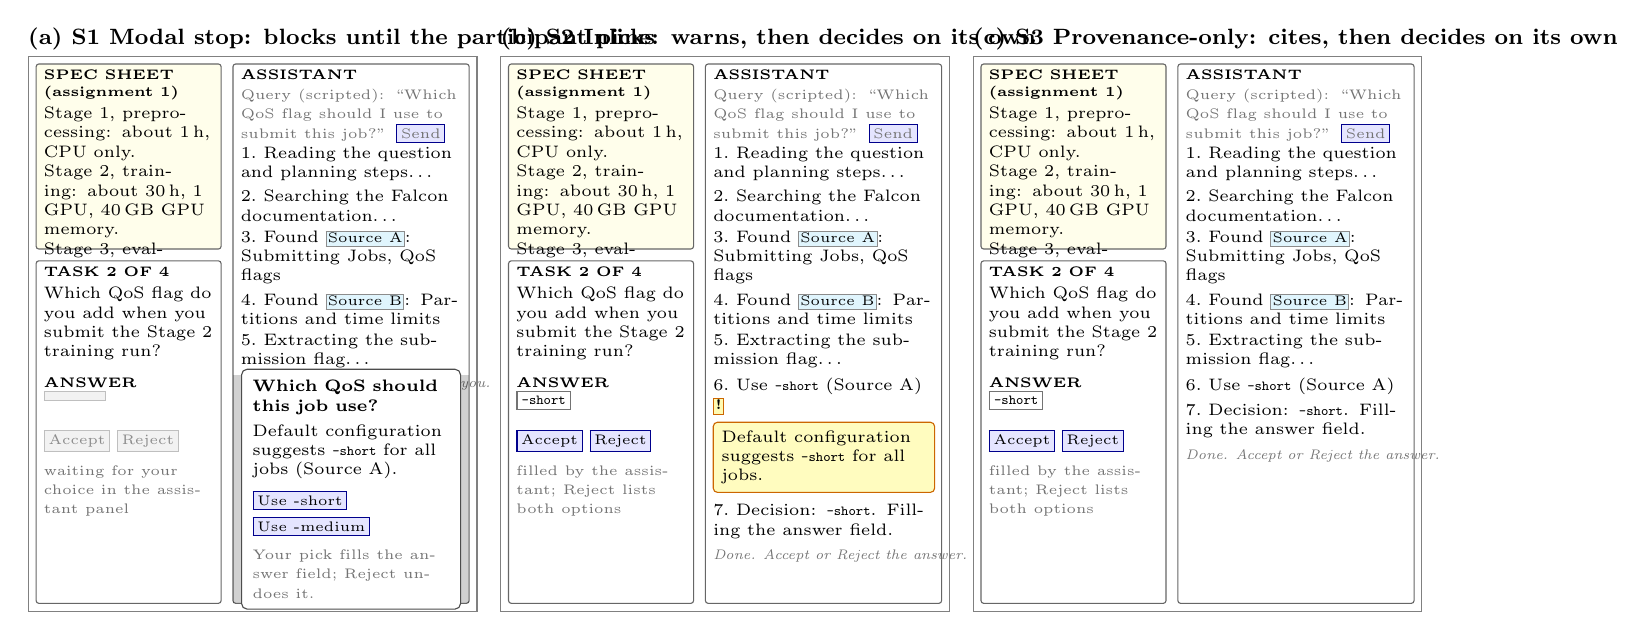
\begin{tikzpicture}[x=1cm, y=1cm, every node/.style={inner sep=0pt, outer sep=0pt, font=\mf}]
% ---- common panel drawing
\newcommand{\basepanel}[2]{% #1 = 1 if answer field is waiting (S1), 0 if autofilled; #2 = label
  \draw[black!50, line width=0.4pt] (0,0) rectangle (5.7,-7.05);
  \node[anchor=south west, font=\footnotesize\bfseries] at (0,0.08) {#2};
  % spec sheet
  \draw[black!60, fill=yellow!8, rounded corners=1pt] (0.1,-0.1) rectangle (2.45,-2.45);
  \node[anchor=north west, text width=2.15cm, align=left] at (0.2,-0.18)
    {\mfs\textbf{SPEC SHEET (assignment 1)}\\[1pt]\mf
     Stage 1, preprocessing: about 1\,h, CPU only.\\
     Stage 2, training: about 30\,h, 1 GPU, 40\,GB GPU memory.\\
     Stage 3, evaluation: about 20\,min, 1 GPU, 8\,GB.\\
     Output is scratch you can regenerate.};
  % task card
  \draw[black!60, fill=white, rounded corners=1pt] (0.1,-2.6) rectangle (2.45,-6.95);
  \node[anchor=north west, text width=2.15cm, align=left] at (0.2,-2.68)
    {\mfs\textbf{TASK 2 OF 4}\\[1pt]\mf Which QoS flag do you add when you submit the Stage 2 training run?\\[4pt]
     \mfs\textbf{ANSWER}};
  \ifnum#1=1
    \node[anchor=north west] at (0.2,-4.25) {\fldg{\hphantom{-medium}}};
    \node[anchor=north west] at (0.2,-4.75) {\btng{Accept} \btng{Reject}};
    \node[anchor=north west, text width=2.1cm, align=left] at (0.2,-5.2)
      {\mfs\color{black!55}waiting for your choice in the assistant panel};
  \else
    \node[anchor=north west] at (0.2,-4.25) {\fld{-short}};
    \node[anchor=north west] at (0.2,-4.75) {\btn{Accept} \btn{Reject}};
    \node[anchor=north west, text width=2.1cm, align=left] at (0.2,-5.2)
      {\mfs\color{black!55}filled by the assistant; Reject lists both options};
  \fi
  % assistant pane frame
  \draw[black!60, fill=white, rounded corners=1pt] (2.6,-0.1) rectangle (5.6,-6.95);
  \node[anchor=north west] at (2.7,-0.18) {\mfs\textbf{ASSISTANT}};
  \node[anchor=north west, text width=2.8cm, align=left] at (2.7,-0.42)
    {\mfs\color{black!55}Query (scripted): ``Which QoS flag should I use to submit this job?'' \btn{Send}};
  \node[anchor=north west, text width=2.8cm, align=left] (t1) at (2.7,-1.15)
    {\mf 1.\ Reading the question and planning steps\ldots};
  \node[text width=2.8cm, align=left, below=1.2mm of t1.south west, anchor=north west] (t2)
    {\mf 2.\ Searching the Falcon documentation\ldots};
  \node[text width=2.8cm, align=left, below=1.2mm of t2.south west, anchor=north west] (t3)
    {\mf 3.\ Found \chip{Source A}: Submitting Jobs, QoS flags};
  \node[text width=2.8cm, align=left, below=1.2mm of t3.south west, anchor=north west] (t4)
    {\mf 4.\ Found \chip{Source B}: Partitions and time limits};
  \node[text width=2.8cm, align=left, below=1.2mm of t4.south west, anchor=north west] (t5)
    {\mf 5.\ Extracting the submission flag\ldots};
}
% ================= panel (a): S1 modal stop
\begin{scope}
\basepanel{1}{(a) S1 Modal stop: blocks until the participant picks}
\node[below=1.2mm of t5.south west, anchor=north west] (pause)
  {\mfs\itshape\color{black!55}Paused at step 6. Waiting for you.};
% overlay (sources above remain clickable)
\fill[black, fill opacity=0.18] (2.6,-4.05) rectangle (5.6,-6.95);
\node[draw=black!70, fill=white, rounded corners=2pt, text width=2.5cm, align=left, inner sep=4pt] at (4.1,-5.5)
  {\mf\textbf{Which QoS should this job use?}\\[2pt]
   Default configuration suggests \mono{-short} for all jobs (Source A).\\[4pt]
   \btn{Use -short}\\[2.5pt]\btn{Use -medium}\\[3pt]
   \mfs\color{black!55}Your pick fills the answer field; Reject undoes it.};
\end{scope}
% ================= panel (b): S2 inline warning
\begin{scope}[xshift=6.0cm]
\basepanel{0}{(b) S2 Inline: warns, then decides on its own}
\node[text width=2.8cm, align=left, below=1.2mm of t5.south west, anchor=north west] (t6)
  {\mf 6.\ Use \mono{-short} (Source A) \wchip{!}};
\node[draw=orange!80!black, fill=yellow!25, rounded corners=1.5pt, text width=2.6cm, align=left, inner sep=3pt, below=1mm of t6.south west, anchor=north west] (flag)
  {\mf Default configuration suggests \mono{-short} for all jobs.};
\node[text width=2.8cm, align=left, below=1.5mm of flag.south west, anchor=north west] (t7)
  {\mf 7.\ Decision: \mono{-short}. Filling the answer field.};
\node[below=1.5mm of t7.south west, anchor=north west]
  {\mfs\itshape\color{black!55}Done. Accept or Reject the answer.};
\end{scope}
% ================= panel (c): S3 provenance-only
\begin{scope}[xshift=12.0cm]
\basepanel{0}{(c) S3 Provenance-only: cites, then decides on its own}
\node[text width=2.8cm, align=left, below=1.2mm of t5.south west, anchor=north west] (t6)
  {\mf 6.\ Use \mono{-short} (Source A)};
\node[text width=2.8cm, align=left, below=1.2mm of t6.south west, anchor=north west] (t7)
  {\mf 7.\ Decision: \mono{-short}. Filling the answer field.};
\node[below=1.5mm of t7.south west, anchor=north west]
  {\mfs\itshape\color{black!55}Done. Accept or Reject the answer.};
\end{scope}
\end{tikzpicture}
\caption{Task 1.2 (Table~\ref{tab:items}) at the fork under the three
forms (wireframes). Left pane: the spec sheet (persistent for the block,
seen only by the participant), the task question, the single answer field
and Accept/Reject. Right pane: the scripted query and the streamed trace.
Lines 1--5, the two source chips, the recommended option and the undo are
identical; only line 6 differs. Under S1 the trace freezes and the modal
blocks the answer field until a pick is made; the chips above the overlay
remain clickable. Under S2 and S3 the assistant fills \texttt{-short} on
its own; they differ only in the warning glyph and recommendation.}
\label{fig:mocks}
\end{figure*}

\subsection{The three forms}
\label{sec:forms}

All three forms share one skeleton: the same trace lines, the same two
source chips printed before the fork, the same recommended option with
the same parenthetical citation, and the same Accept/Reject controls with
one-step undo. This holds MiPP's C1--C3 constant. The forms are defined
by whether the fork is \emph{announced} and whether the task is
\emph{blocked}:
\begin{description}
\item[S1, modal stop (announced, blocking).] The trace freezes at the
decision line. A modal names both options and one brief recommendation
(``Default configuration suggests \texttt{-short} for all jobs''), with a
button for each. Nothing proceeds and the field stays empty until the
participant picks; the field is then filled with the pick.
\item[S2, inline warning (announced, not blocking).] The trace keeps
streaming. The decision line carries a small warning glyph with the same
recommendation sentence beneath it. The assistant takes the recommended
option without waiting, and the field is filled with it.
\item[S3, provenance-only (not announced).] The trace keeps streaming.
The decision line states what was found with a citation (``Use
\texttt{-short} (Source A)''), no glyph, no stated alternative. The
assistant takes the recommended option, and the field is filled with it.
\end{description}
Only S1 requires an action; S2 and S3 proceed automatically and differ
only in whether a warning and recommendation are shown
(Figure~\ref{fig:mocks}). The forms are not MiPP's families, which also
differ in trigger and in whether the system acts before or after asking;
we take MiPP's constraints, not its taxonomy. Provenance-only is current
practice~\cite{ravi2025} and the C5 silence of Section~\ref{sec:related}.
Verification is defined as opening a source from the trace, which no form
forces, so a difference cannot be produced by the modal form requiring a
click; the modal form does force a \emph{choice}, which is inherent to
blocking and reported as such.

\subsection{Why this is an agentic, human-centered study}
\label{sec:agentic}

\begin{figure}[t]
\centering
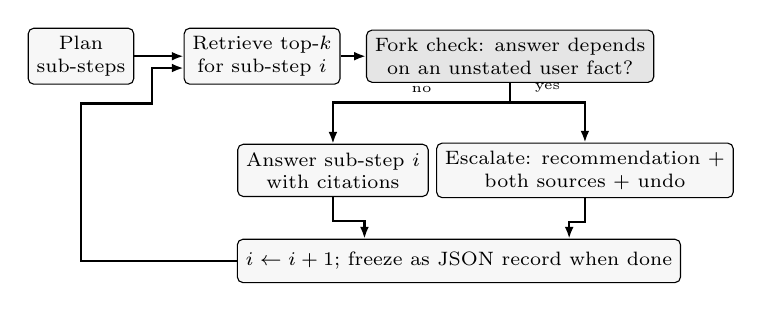
\begin{tikzpicture}[x=1cm, y=1cm,
  box/.style={draw, rounded corners=2pt, align=center, font=\scriptsize,
              minimum height=5.5mm, inner sep=3pt, fill=black!3},
  dec/.style={draw, rounded corners=2pt, align=center, font=\scriptsize,
              minimum height=5.5mm, inner sep=3pt, fill=black!10},
  arr/.style={-{Latex[length=1.5mm]}, thick}
]
\node[box] (plan) at (0,0) {Plan\\sub-steps};
\node[box] (ret) at (2.3,0) {Retrieve top-$k$\\for sub-step $i$};
\node[dec] (chk) at (5.45,0) {Fork check: answer depends\\on an unstated user fact?};
\node[box] (ans) at (3.2,-1.45) {Answer sub-step $i$\\with citations};
\node[box] (esc) at (6.4,-1.45) {Escalate: recommendation $+$\\both sources $+$ undo};
\node[box] (next) at (4.8,-2.6) {$i \leftarrow i+1$; freeze as JSON record when done};
\draw[arr] (plan) -- (ret);
\draw[arr] (ret) -- (chk);
\draw[arr] (chk.south) -- ++(0,-0.25) -| node[above, font=\tiny, pos=0.25] {no} (ans.north);
\draw[arr] (chk.south) -- ++(0,-0.25) -| node[above, font=\tiny, pos=0.25] {yes} (esc.north);
\draw[arr] (ans.south) -- ++(0,-0.3) -| ([xshift=-1.2cm]next.north);
\draw[arr] (esc.south) -- ++(0,-0.3) -| ([xshift=1.4cm]next.north);
\draw[arr] (next.west) -| (0,-1.45) -- (0,-0.6) -- (0.9,-0.6) |- ([yshift=-1.5mm]ret.west);
\end{tikzpicture}
\caption{The loop that drafts each task. The fork check is the
retrieval-score margin plus an LLM judge. Its output is frozen as the
trace and replayed identically to every participant; only the rendering
of the ``Escalate'' line differs between conditions.}
\label{fig:loop}
\end{figure}

Tasks are drafted by a minimal agentic RAG loop (Figure~\ref{fig:loop}):
given the query it plans sub-steps (read, search, extract the flag,
decide), retrieves the top-$k$ chunks per sub-step from the snapshot, and
runs a fork check that fires when the retrieval-score margin between the
top candidates is small \emph{and} an LLM judge answers yes to ``do these
chunks give different answers depending on a user attribute the query
does not state?'' For the running example the check fires at the
extraction sub-step, where the top chunks are the \texttt{-short} and
\texttt{-medium} entries with different wall-time limits and the query
names no run length. Only queries on which the check fired become tasks;
we report its hit rate. Each task is then frozen as a JSON record (sheet
line, query, trace lines with source ids, fork line index, the two
options, recommended option, key), and the web app reads only the record,
so every participant sees identical content and the flag changes only the
fork line's rendering.

\emph{Pre-generated, replayed behavior.} Agent behavior is generated by the
pipeline before the sessions and replayed identically to every participant,
following the fixed-advice paradigm common in AI-reliance
studies~\cite{bucinca2021,vasconcelos2023,schemmer2023}\verify{} and the
older practice of controlling system behavior in intelligent-interface
studies~\cite{dahlback1993}\verify{}, so that escalation points,
recommendations and their correctness are controlled. The pipeline runs
locally on an open-weight model at temperature 0 with a fixed seed; the
snapshot, task records, fork-check log and model digests are released.
Authors may edit wording but never an escalation decision or a
recommendation; recommendation correctness is set by the sheet line, not
by overriding the agent. Participants are told the assistant's responses
were prepared in advance. The study thus isolates the human-facing form of
an agent-initiated escalation, not the agent's behavior or multi-turn
interaction.

This passes the ``if a chatbot can do it'' test: a chatbot
answers the query as asked, and only a loop that retrieves per step and
inspects its own retrieval can discover mid-task that the answer depends on
an unstated fact and choose to hand the decision back. The human-centered
question is what that hand-back should look like, and every outcome is a
human behavior. ``Agentic'' rests on four properties, each verifiable in
the released records: the task is multi-step, the escalation arrives at
the affected step, the trigger is the loop's own decision, and the loop is
fully described here. If any fails in the built system we will call it a
RAG assistant with system-initiated escalation.

\subsection{Corpus and tasks}
\label{sec:corpus}

% Corpus sections are not final. Requirements below are fixed.
The corpus is a frozen snapshot of the CSU CS department systems
documentation for the Falcon cluster (sna.cs.colostate.edu); which
sections are used is not yet decided. Requirements are fixed: every key
derivable from the snapshot plus one sheet line, with no administrator
verification; snapshot and task records released together; 12 measured
tasks in three sets of four, each set from a disjoint section (job
submission; access and remote connection; storage and software), plus 2
practice tasks; and a system many CSU students have not used. Each set is
two fork source-pairs used twice each, once with the recommended option
correct and once wrong, and no source pair recurs across sets.
Table~\ref{tab:items} gives illustrative tasks written against the current
pages. We keep the FictionalQA blind-versus-informed
check~\cite{kirchenbauer2026} as a filter: the drafting model is queried
blind and with the two sources, and facts it answers correctly blind are
discarded (department-local hostnames, QoS names and paths are the kind
that fail blind). Task sets are matched on trace length, fork line index,
query--source lexical overlap band and fork type, checked in the pilot,
and task is a random effect in every model. Because someone who already
knows the \texttt{-short} limit could resolve task 1.2 without opening a
source, we screen for prior use, prefer forks whose condition is stated
only on the page, and log what was opened.

\textbf{No control tasks.} The previous draft added two no-fork control
tasks per block, for a baseline page-opening rate and so that two
citations never signalled a fork. Both purposes are moot here: every trace
cites Source A and Source B, so two citations carry no signal, and the
baseline that matters for H1 is the provenance-only form itself, in which
nothing announces the fork. Cutting them is a deliberate simplification:
it costs a within-participant estimate of spontaneous source opening with
no fork present, which none of H1--H3 needs, and buys a shorter block, a
longer trace per task, and one scored field instead of a card of decoy
dropdowns. The fork base rate is therefore 100\% in every block and is
disclosed up front (Section~\ref{sec:eval}).

\begin{table}[t]
\centering\scriptsize
\caption{Illustrative tasks from the Falcon documentation. The set tied to
S1 is shown in full (two source pairs, each used once correct and once
wrong); for the other sets one wrong-recommendation task is shown, and
its correct twin uses the same sources with a different sheet line. Page
facts are from the current pages; the pairing is illustrative until the
snapshot is frozen.}
\label{tab:items}
\begin{tabular}{@{}>{\raggedright\arraybackslash}p{0.045\linewidth}>{\raggedright\arraybackslash}p{0.30\linewidth}>{\raggedright\arraybackslash}p{0.33\linewidth}>{\raggedright\arraybackslash}p{0.19\linewidth}@{}}
\toprule
\textbf{ID} & \textbf{Task question (sheet line that decides it)} & \textbf{Source A / Source B and the two options} & \textbf{Recommended $\rightarrow$ key} \\
\midrule
\multicolumn{4}{@{}l}{\emph{Set tied to S1: job submission. Assignment: fine-tune a model in three stages.}} \\
1.1 & QoS flag for the Stage 1 preprocessing job (about 1\,h). & Submitting Jobs, QoS flags / Partitions and time limits: \texttt{-short} vs.\ \texttt{-medium}. & \texttt{-short} (correct) \\
\addlinespace
1.2 & QoS flag for the Stage 2 training run (about 30\,h). & Same sources and options. & \texttt{-short} (wrong) $\rightarrow$ \texttt{-medium} \\
\addlinespace
1.3 & GPU partition for the Stage 2 training run (40\,GB GPU memory). & GPU Jobs / Partitions: RTX 3090 (24\,GB) partition vs.\ A100 (40/80\,GB) partition. & 3090 partition (wrong) $\rightarrow$ A100 partition \\
\addlinespace
1.4 & GPU partition for the Stage 3 evaluation (8\,GB GPU memory). & Same sources and options. & 3090 partition (correct) \\
\midrule
\multicolumn{4}{@{}l}{\emph{Set tied to S2: access and remote connection. Assignment: set up the course project from home and from the lab.}} \\
2.1 & First step to connect (you are at home; twin 2.2: at a CS lab machine). & Connecting to Falcon: \texttt{ssh falcon.cs.colostate.edu} / SSH guide: off campus, connect to the CSU VPN first. & ssh directly (wrong) $\rightarrow$ VPN, then ssh \\
\midrule
\multicolumn{4}{@{}l}{\emph{Set tied to S3: storage and software. Assignment: prepare data and environment for the project.}} \\
3.1 & Where the job writes its output (scratch you can regenerate; twin 3.2: the final model, which must be kept). & Home Directories: home (backed up, quota) / Temporary Disk Space: \texttt{/s/<host>/a/tmp} (not backed up, scrubbed). & home (wrong) $\rightarrow$ \texttt{/s/<host>/}\allowbreak\texttt{a/tmp} \\
\bottomrule
\end{tabular}
\end{table}
% TODO authors: verify -- the second source pair for the S2 and S3 sets
% (tasks 2.3-2.4 and 3.3-3.4) must come from the drafting pipeline once the
% snapshot is frozen; do not hand-seed them.
% TODO authors: confirm -- task sets are tied to systems as agreed on the
% whiteboard, so set and form are confounded. Crossing set with form (as in
% v3's Latin square of set x form) removes this at no extra cost; if you keep
% the tie, the matching procedure and the task random effect are the only
% defenses and Threats says so.

\section{System Vision and Technology}
\label{sec:vision}

The apparatus is one web application (React or plain JavaScript) with a
condition flag, run in a desktop browser with no headset or spatial
component. The screen has the two panes of Figure~\ref{fig:mocks}. A
replay engine reads the task's JSON record and prints the trace at a fixed
3--5\,s per line; the flag selects one of three renderings of the fork
line and nothing else. Clicking a source chip opens the frozen passage in
an overlay over the trace with the relevant lines highlighted; a close
control returns to the trace, and under S1 the chips stay active while
the modal is up. Every interaction is logged as a timestamped event
(block, form, task, Send, each trace line onset, fork onset, modal pick,
each source opened and closed, autofill, Accept, Reject, picker choice,
final value, block boundaries) to a local SQLite database under a
participant code.
Instruments appear as full-screen steps between blocks. The drafting
pipeline is Python: the snapshot is chunked by heading, embedded into a
vector index, and queried per sub-step; one LLM plans sub-steps and acts
as the fork judge. The model will be named in the paper; because records
are frozen, the human-facing study does not depend on it. We estimate one
week for the pipeline and two for the web application.

\section{Evaluation Plan}
\label{sec:eval}

\paragraph{Participants.}
CSU students who have not used Falcon (screening item), recruited through
the class data-collection form; the realistic pool is upper-division
undergraduates and new graduate students. $N{=}18$ target (three per block
order), 12 minimum (two per order); pilot of 3--4 not included. The class
form suffices for the course; if we intend to publish, an IRB protocol
with a faculty principal investigator is needed before recruitment, and we
will raise it with the instructor in the first two weeks of October.

\paragraph{Design.}
\emph{Independent variables:} (1) Escalation Form, three levels, S1 modal
stop, S2 inline warning, S3 provenance-only; within subjects, one level
per block. (2) Recommendation Correctness, two levels, correct and wrong,
defined per task by whether the recommended option equals the key derived
from the spec sheet; within subjects, two tasks per level in every block,
randomized within block. \emph{Nuisance variable:} Block Order, the six
permutations of (S1, S2, S3), between subjects, assigned in rotation;
order is the only thing that differs between groups. \emph{Design
statement:} a $3\times2$ within-subjects factorial, Escalation Form
$\times$ Recommendation Correctness, two replicates per cell per
participant: 12 tasks per participant (6 correct-recommendation, 6 wrong)
and, at $N{=}18$, 216 tasks and 36 per cell. Each form's block carries
its own fixed set of four tasks (Table~\ref{tab:items}). A
between-subjects design would need roughly three times as many people for
the same power, which at class scale leaves four to six per condition, so
we keep within subjects.

\emph{Dependent variables}, per task unless stated: (a) \emph{Verified},
binary, at least one of the two fork sources opened from the trace between
Send and the final Accept. (b) \emph{Source pattern}, four-level: the
recommended source only (the one cited on the decision line), the
non-recommended only, both, or neither; and \emph{Dwell}, seconds each
source was open, summed over openings. (c) \emph{Followed}, binary, final
value equals the recommended option; crossed with Recommendation
Correctness this gives the four cells of appropriate reliance, following a
correct recommendation and overriding a wrong one being
appropriate~\cite{schemmer2023}, from which relative AI reliance and
relative self-reliance follow. (d) \emph{Accuracy}, binary, final value
equals key. (e) \emph{Decision time}, seconds from onset of the fork line
(or modal) to the final Accept; the scripted preamble is identical within
a task and is excluded. (f) Per block: raw NASA-TLX, one
perceived-intrusion item (1--7, as in MiPP-Eval, for comparability) and a
manipulation check (identify the form just used). (g) Per session: a
ranking of the three forms and a free-text reason. Nothing else is
collected. Verified is the primary verification measure, for continuity
with the binary hypothesis; Source pattern and Dwell are secondary and
reported descriptively by form.

\paragraph{Procedure.}
A session takes about 45 minutes. (1)~Consent and instructions, 5\,min.
The participant reads the cover story: ``You are a student using the
Falcon cluster for an assigned project. You are given the assignment
details and an agentic AI assistant for the cluster documentation that
retrieves from those documents. You will complete a series of tasks
derived from the assignment.'' The instructions state that the assistant
is usually right but can be wrong, that the spec sheet describes their
assignment, and that they may open any source the assistant cites.
(2)~Practice, 3\,min: two tasks on a practice sheet with no fork; the
trace cites two agreeing sources and fills the field, and the
experimenter has the participant open and close a source and use Reject
and Accept once each. These are the only unforked tasks and are not
scored. (3)~Three measured blocks, about 9\,min each. At the start of a
block the sheet for that block's assignment replaces the previous one and
stays on screen; the block's four tasks then run in random order through
the loop of Section~\ref{sec:trial}, and the block ends with raw
NASA-TLX, the intrusion item and the manipulation check as full-screen
steps. (4)~Closing questionnaire, 5\,min: the ranking and its reason.
Every deciding fact appears on exactly one sheet line and is tested by
exactly one task. Block position enters the models as a covariate and the
first block is reported alone as a descriptive between-subjects check.

\paragraph{Hypotheses.}
\textbf{H1 (verification).} The proportion of tasks with Verified $=1$ is
ordered S1 $>$ S2 $>$ S3; the tested contrasts are S1 vs.\ S2 and S2 vs.\
S3, each one-sided. Secondary, descriptive: Dwell on the non-recommended
source follows the same order. \textbf{H2 (appropriate reliance).} On
wrong-recommendation tasks the override rate, $P(\text{Followed}=0)$, is
higher under S1 and under S2 than under S3; on correct-recommendation
tasks the follow rate, $P(\text{Followed}=1)$, does not differ across
forms. Together these are a Form $\times$ Correctness interaction on
Followed, with the form effect confined to wrong-recommendation tasks.
\textbf{H3 (cost).} Decision time per task and raw NASA-TLX per block are
ordered S1 $>$ S2 $>$ S3. H1 and H3 together are the trade-off reported
for forcing functions~\cite{bucinca2021}; H2 is what matters to a
designer. The ranking is reported descriptively.

\paragraph{Analysis.}
Primary analyses are at the task level (four tasks per form per
participant, two per cell): logistic mixed models for Verified and for
Followed, with fixed effects of form, correctness, their interaction and
block position, and random intercepts for participant and task; a linear
mixed model on log decision time; repeated-measures ANOVA with
Greenhouse--Geisser correction, or Friedman, for TLX and intrusion.
Planned contrasts (S1 vs.\ S2, S2 vs.\ S3) are Holm-corrected and reported
as odds ratios or $d_z$ with 95\% CIs. Source pattern is reported as a
form $\times$ pattern contingency table with Dwell medians. Free-text
reasons are coded thematically by both authors. A paired $t$-test at
$N{=}12$ detects only large participant-level effects ($d_z \approx 0.9$
at 80\% power), which is why task-level models are primary; we will
simulate power for the H2 interaction from pilot estimates.

\paragraph{Threats.}
Strategy carry-over (learning that every task hides a fork) is addressed
by the up-front instruction, all six orders, the position covariate and
the first-block check; the fork base rate is 100\% in every block, so
carry-over cannot favor one form. Task set and form are confounded by the
fixed tie between each form and its four tasks; the matching procedure,
the disjoint sections and the task random effect are the defenses, and the
confound is stated as a limitation. Domain knowledge that resolves a fork
without opening a source (including guessing from the flag names) is
addressed by screening, by keying on limits stated only on the page, and
by logs. Forced choice under S1 is inherent to blocking; verification is
never forced, and under S1 the chips stay reachable while the modal is up.
Generality is limited to one corpus, novices, a short lab session and
replayed single-turn sessions without follow-up questions, and is stated
as a scope condition.

\section{Deliverables}
\label{sec:deliverables}

\textbf{By mid-November:} the frozen snapshot of the chosen sections; the
drafting pipeline with its fork check and a log of where it fired over
about 30 candidate queries; the contamination-filter survivor count; 12
measured and 2 practice task records assembled into three matched sets of
four; three spec sheets; the web application with the three renderings,
replay engine, source overlay, instruments and event logging; a completed
pilot of 3--4 people with tasks and timing revised; and the IRB decision.
\textbf{By the early-December presentations:} 12--18 completed sessions;
the analysis scripts and results for H1--H3; a paper draft with Method and
Results; a demo video of one task in all three forms; and the released
snapshot plus task records. The critical path is task authoring, not code.

\textbf{Team.} Group CS567\_Coen\_Cam\_Context\_Not\_Found. Coen Petto:
study design, web application and participant sessions. Cameron Suess:
drafting pipeline, task authoring and corpus snapshot. Both authors write
and analyze.
% TODO authors: confirm roles

\section{Conclusion}

We propose a within-subjects study of how an agentic RAG assistant should
hand a decision back when the right answer depends on a fact about the user
it was never told. The agent, its escalation points and its provenance are
held constant; only the form varies, and the recommendation is wrong for
this participant on half of the tasks, so verification has a payoff. The
prediction is that a modal stop buys the most verification at the highest
cost, that an inline warning captures most of the benefit for less, and
that a provenance-only citation, which is what current RAG interfaces
provide and what MiPP's C5 counsels, leaves the agent's errors largely
uncaught. Whichever way the results fall, they answer a question that
MiPP, the agentic-RAG pattern and the reliance literature each pose and
none has tested.

\section*{Use of AI}

Claude Code (Anthropic), running Claude Opus 5.5 with Claude Fable 5.1
subagents, was used in preparing this checkpoint to: critique the
instructor's feedback and the original proposal; read the full text of the
MiPP paper and check our claims against it; check each bibliographic entry
against publisher records (Crossref, IEEE Xplore, Springer, ACM, ICLR
proceedings, arXiv) and produce corrected BibTeX; draft the text of this
document; and draw the TikZ mock-ups. A further pass with Claude Code
(Claude Fable 5.1) rewrote the draft to this version from our whiteboard
notes, which fixed the Falcon \texttt{-short}/\texttt{-medium} example,
the spec sheet, the per-task trace and the 12-task design, and redrew the
mock-ups to match; the bibliography was not changed in that pass. The
authors made every design decision, revise the text, and verify each
reference on the publisher page before submission; fields the tool could
not confirm are marked with a ``verify'' comment in the source and omitted
until confirmed.
% TODO authors: verify -- add any other AI tools used on the original
% proposal (for example, for grammar or LaTeX fixes) and what each did.

%% ---------------------------------------------------------------- references
\bibliographystyle{ACM-Reference-Format}
\bibliography{references}

\end{document}
